\documentclass[12pt]{article}
\setlength{\oddsidemargin}{27mm}
\setlength{\evensidemargin}{27mm}
\setlength{\hoffset}{-1in}

\setlength{\topmargin}{27mm}
\setlength{\voffset}{-1in}
\setlength{\headheight}{0pt}
\setlength{\headsep}{0pt}

\setlength{\textheight}{235mm}
\setlength{\textwidth}{155mm}

%\pagestyle{empty}
\pagestyle{plain}

\renewcommand{\thefootnote}{\fnsymbol{footnote}}
\renewcommand{\labelitemi}{$\diamond$}

\usepackage{cite}
\usepackage{amsmath}
\usepackage{amsfonts}
\usepackage{amssymb}
\usepackage{graphicx}
\usepackage{multirow}
%\usepackage{algpseudocode}

\begin{document}
\baselineskip 12pt

\begin{center}
\textbf{\Large Predicting Machine Failures with Reinforcement Learning}

\vspace{1.5cc}
{ \sc Dalton Schutte}\\

\vspace{0.3 cm}

{\small Georgia Institute of Technology}
\end{center}
\vspace{1.5cc}



\begin{abstract}
  \noindent We investigate methods from statistical process control, deep learning, and reinforcement learning
  for predicting when two machines will fail. Each machine is fitted with sensors that report data at semi-regular
  intervals for each time step. Our results suggest that there is promise in reinforcement learning agents trained
  using proximal policy optimization. Our findings also suggest that there is value in daily generated T$^2$ control
  charts. The state of the art time series transformer model could not be trained so we do not make an assessment of
  its abilities, however, given the nature of the model it may be worth additional troubleshooting to evaluate its
  potential. Ultimately, the control charts are likely the best performance to cost option due to the lower compute, 
  expertise, and data availability they require.
\end{abstract}



\section{Introduction} \label{form}

As time progresses, machines gradually wear down and will fail. When a machine fails,
it is likely to require maintenance or repair before it can return to its normal function.
Depending on the application, failure may not be an issue if the process is low-stakes or
has redundancies or backups or catastrophic if the process is of critical importance. In
most cases, machine failure may result in lost revenue as production is halted or goods
are damaged.

Knowing when a machine is likely to fail can reduce the impact on down- and up-stream
processes by allowing necessary preparations to be taken before the machine is stopped
for maintenance. This is preferable to the alternative where the failure remains unaddressed
until it is noticed. This can add to down times and makes preparing for the downtime 
rushed.

\subsection{Background} \label{back}

\subsubsection{Statistical Process Control}

Statistical Process Control (SPC), or, Statistical Quality Control, is a set or techniques
that allow one to track the results of a process over time\cite{guthrie_nistsematech_2020}. 
The general procedure is:

\begin{enumerate}
    \item Determine which time period will be used for establishing in-control markers
    \item Gather observations from this period
    \item Calculate the center line
    \item Calculate any control limits (such as 2 standard deviations above/below the center line)
    \item Plot new observations against these limits
    \item Evaluate any patterns that emerge
\end{enumerate}

There are different types of charts depending on what observations are available, the nature
of the process, etc. Typically, a single characteristic is measured (e.g. weight for canned goods,
length of extruded metal, etc.) per chart for simplicity. Tracking multiple variables is
complex and requires special methodologies.

\subsubsection{Deep Learning}
Deep learning is a procedure where deep neural networks are trained on a dataset using an
optimization algorithm in an iterative manner. There are many flavors of neural network, but
two that are particularly well suited to sequential data are the Long-Short Term Memory (LSTM)
network\cite{hochreiter_long_1997} and the transformer\cite{vaswani_attention_2023}.

Transformer-based architectures have been at the forefront of NLP research in recent years. While they have
demonstrated excellent performance on some generative language tasks, their ability to process long-term
dependencies in sequential data and the ability to pre-train models once and fine-tune for multiple other tasks
suggests they could be well suited to applications in time series analysis. Indeed there has been some research
on this front. Recently Goswami et al.\cite{goswami_moment_2024} collected a large amount of time series data
to pre-train a family of models called MOMENT. This family of foundational time series models is pre-trained
on time series from a variety of domains, with varying time horizons, and for various tasks.

\subsubsection{Reinforcement Learning}
Reinforcement learning (RL) is a special subset of ML/AI focused on choosing actions in some environment\cite{sutton_reinforcement_1998}.
This process begins with some "agent" that will use some reinforcement learning algorithm to
interact with an environment which, in turn, provides a reward signal that is used to help
train the agent. The ultimate goal is for the agent to learn an optimal policy, $\pi$, that
can be used to choose actions given a state. Perhaps one of the most famous applications of
reinforcement learning is in games. Many board games, such as Go\cite{silver_mastering_2017},
have a huge number of discrete game states that one cannot simply find the best play with brute
forced.

Two of the, perhaps, most well-known techniques are Proximal Policy Optimization (PPO)\cite{Schulman2017ProximalPO} and
Neural Guided Monte Carlo Tree Search (MCTS)\cite{silver_mastering_2016}. The former was used to train the OpenAI 5, a 
collection of AI agents trained to play the video game Dota 2\cite{Berner2019Dota2W} and the latter to train AlphaGo,
which beat the then Go world champion in a set of 4-1.

\subsection{Research Questions}
The states for many machine sensors are not discrete, but rather, take on values in $\mathbb{R}$.
The T$^2$ and, most, deep learning models handle this situation without issue. There are plenty
of RL algorithms that can solve continuous control tasks\cite{Pong2018TemporalDM,Lillicrap2015ContinuousCW}.
However, we wish to examine the efficacy of RL for stopping machines that are about to fail. We
will seek to answer the following questions:

\begin{enumerate}
    \item How well can MCTS and PPO perform at this task?
    \item How do these algorithms compare to traditional methods from SPC?
    \item How do these algorithms compare to models, such as MOMENT, designed for sequential data?
    \item How do the RL methods compare to each other?
\end{enumerate}


\section{Methods} \label{meth}
\subsection{Data}

We are using data from two machines, a blood refrigerator and a nitrogen generator\cite{pinciroli_vago_predicting_2024}.

A blood refrigerator is a machine designed to store blood safely at proper temperatures. The general composition of a unit
is the compressor to pump coolant throughout, the condensor to remove heat from the collant and condense it, the
evaporator which evaporates the coolant to cool the interior of the unit, an expansion valve to regulate the flow of
coolant, and tubing to move the coolant throughout.

A nitrogen generator is a machine that separates nitrogen from other gases in compressed air. This unit typically includes an
air compressor, carbon sieves for filtering, absorption vessels to collect nitrogen, and towers to increase production.

\subsubsection{Analysis}

\begin{table}[b]
    \centering
\begin{tabular}{l|ll|ll|}
\cline{2-5}
                                & \multicolumn{2}{l|}{Blood Refrigerator} & \multicolumn{2}{l|}{Nitrogen Generator} \\
                                & Train              & Test               & Train              & Test               \\ \hline
\multicolumn{1}{|l|}{Days}      & 25                 & 27                 & 29                 & 8                  \\
\multicolumn{1}{|l|}{Timesteps} & 60166              & 65763              & 40354              & 11162              \\
\multicolumn{1}{|l|}{Stops (1)} & 704                & 642                & 810                & 242                \\ \hline
\end{tabular}
\caption{Summary statistics of our datasets}
\end{table}

The data includes a mix of binary and continuous variables with a binary target variable. The class imbalance is heavily in
favor of the 'normal' class \text{(PW\_0.5h=0)}, which indicates the machines are operating within expecations the majority of the time,
a desireable phenomenon. The ratio of normal to failed states is roughly 99:1 for the blood refrigerator and 49:1 for the nitrogen
generator. In each dataset, there are several days where there is no failure state, meaning the machine operated without issue
the entire day.

The measurement intervals are spaced roughly 1 minute apart for the nitrogen generator and about 34 seconds for the blood refrigerator.
The label \text{'PW\_0.5'}, using the notation and convention from the paper
that provided this dataset\cite{pinciroli_vago_predicting_2024}, represents the Prediction Window \text{(PW)} of 30 minutes \text{(0.5 hours)}.
This means that in the 30 minute interval beginning at a time stamp $t$, the machine is operating outside of parameters for at least
one of those time stamps. The other convention from that paper is the Reading Window over some interval. The Reading Window \text{(RW)} is
the collection of sequential time stamps used as input to a model. In our experiments, for example, we use a RW of 20 minutes where
we collect the minimum number of sequence of time steps necessary to span 20 minutes of time. In Pinciroli et al.\cite{pinciroli_vago_predicting_2024},
they explore a wide combination of PW and RW but found that most of their models performed best with a 20 minute RW, which is why
that is the window size we chose to use.

\begin{figure}
    \centering
    \includegraphics[width=16cm]{assets/test/blood-refrigerator/features.png}
    \caption{Plots of variables around the point of failure for the blood refrigerator. Red regions are where regions where the data label indicates failure (1)}
    \centering
    \includegraphics[width=16cm]{assets/test/nitrogen-generator/features.png}
    \caption{Plots of variables around the point of failure for the nitrogen generator. Red regions are where regions where the data label indicates failure (1)}
\end{figure}

Figures 1 and 2 show some examples of the time series data in our dataset. Initially, the blood refrigerator dataset had 16 sensors
providing output and the nitrogen generator had 7. We removed all the output from any sensor whose standard deviation was zero over
the entire dataset. This left 12 variables for the blood refrigerator and 4 for the nitrogen generator.

The time series for the features in the blood refrigerator (figure 1) highlight that there is, intuitively, some change occurring
in the machine that is leading to these sensor readings. Particularly, the product temperature base, evaporator temperature, and power
supply have noticeably different patterns in the red failure region than in the period before.

The nitrogen generator (figure 2) shows an instance where the failure happens early in the observation period, only a few time steps
into the beginning of the period. This poses a challenge for the methods as there is very little data for them to work from before having
to determine if the machine is on a trajectory to failing. However, this may be the case in real operating conditions and so is an
important case to keep in our dataset.

\paragraph{Correlations}

\begin{figure}[h]
    \centering
    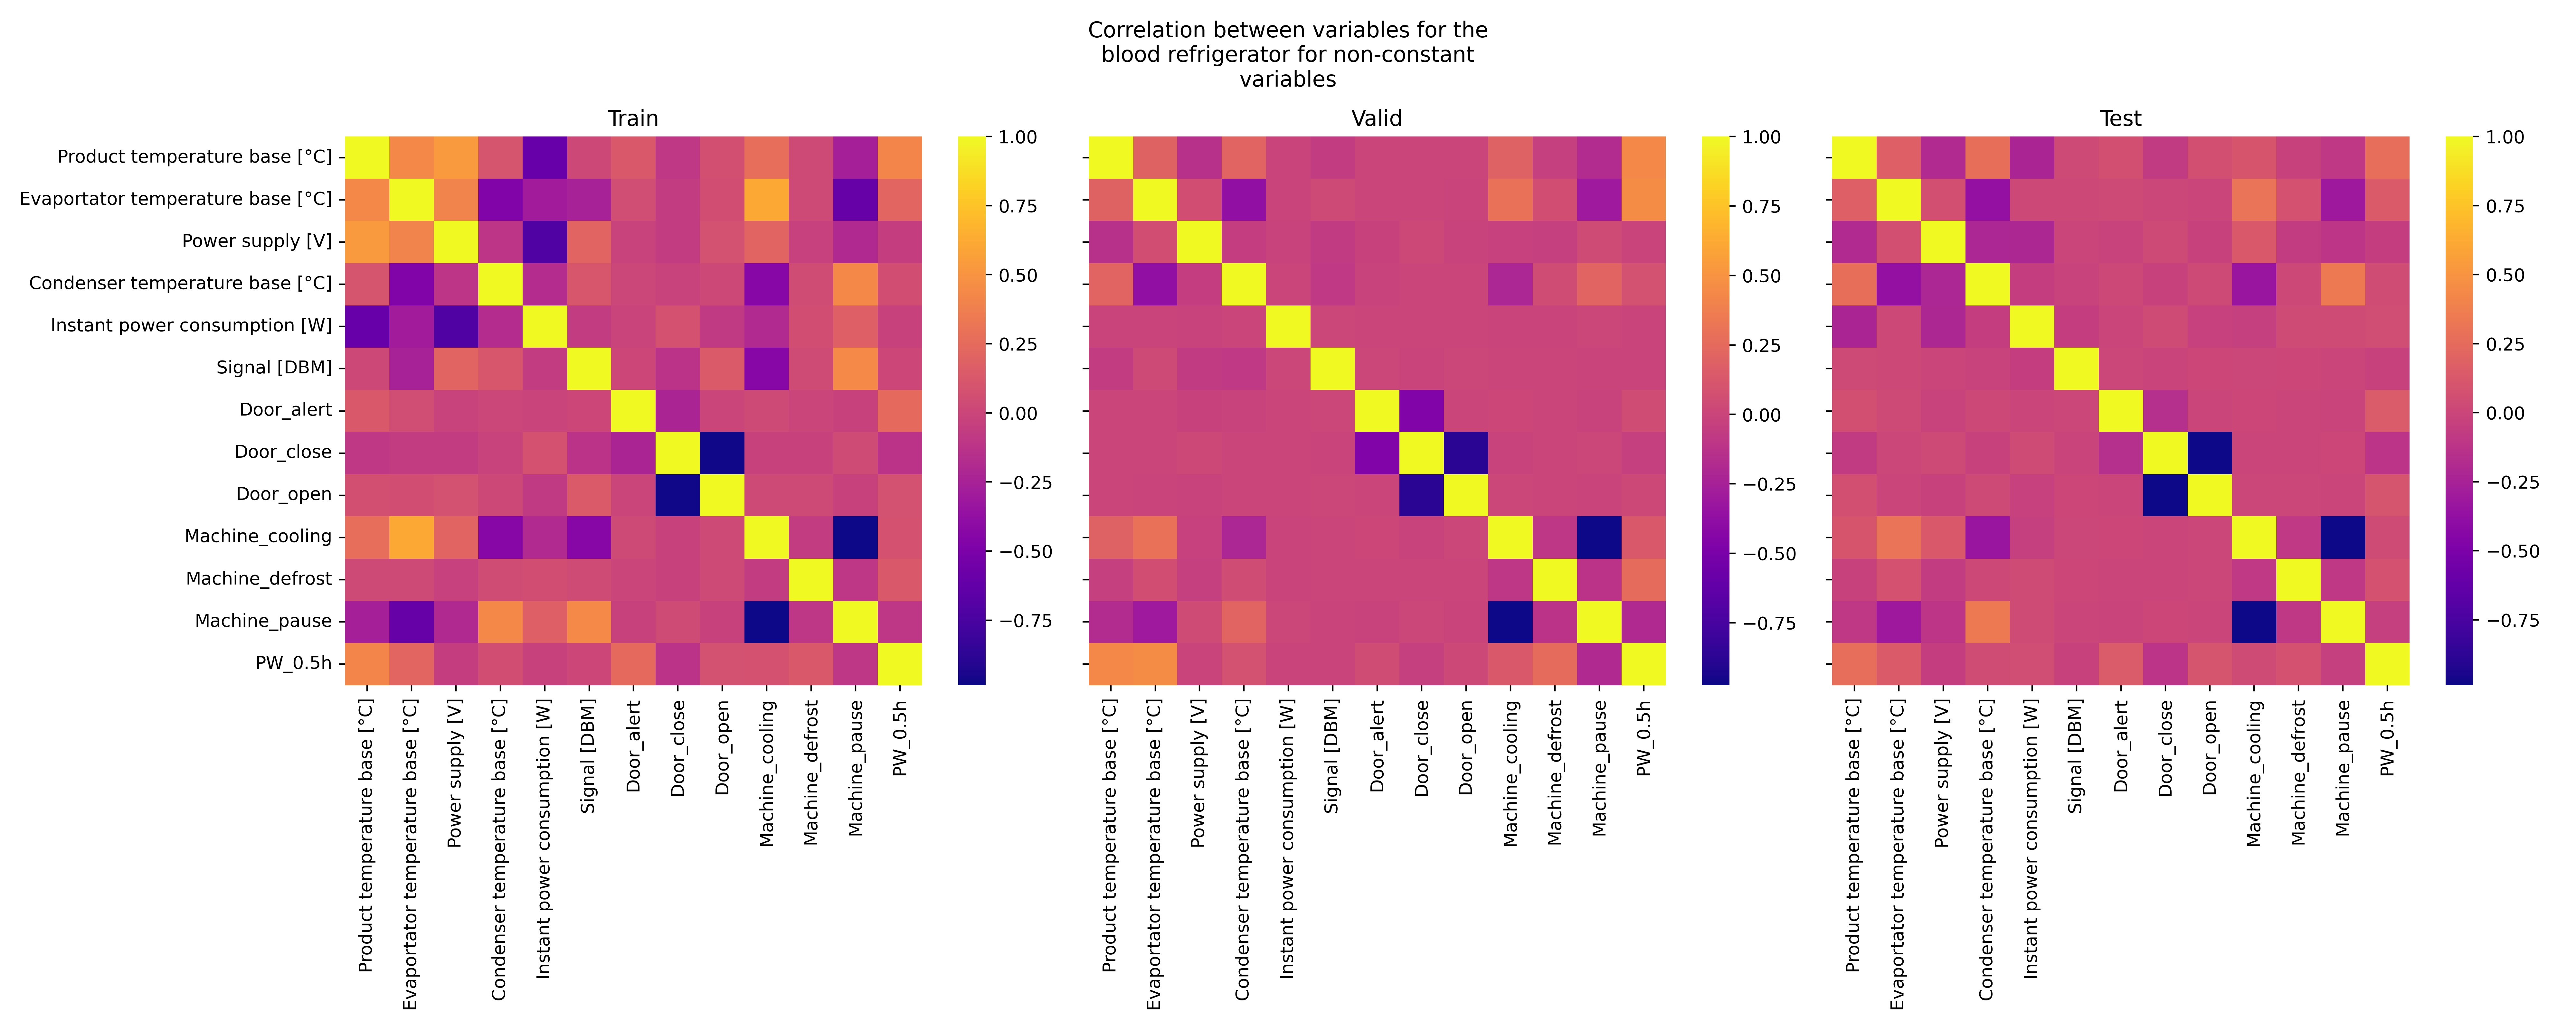
\includegraphics[width=16cm]{assets/test/blood-refrigerator/correlations.png}
    \caption{Correlation between variables in the blood refrigerator dataset splits. The label column is 'PW\_0.5h'.}
    \centering
    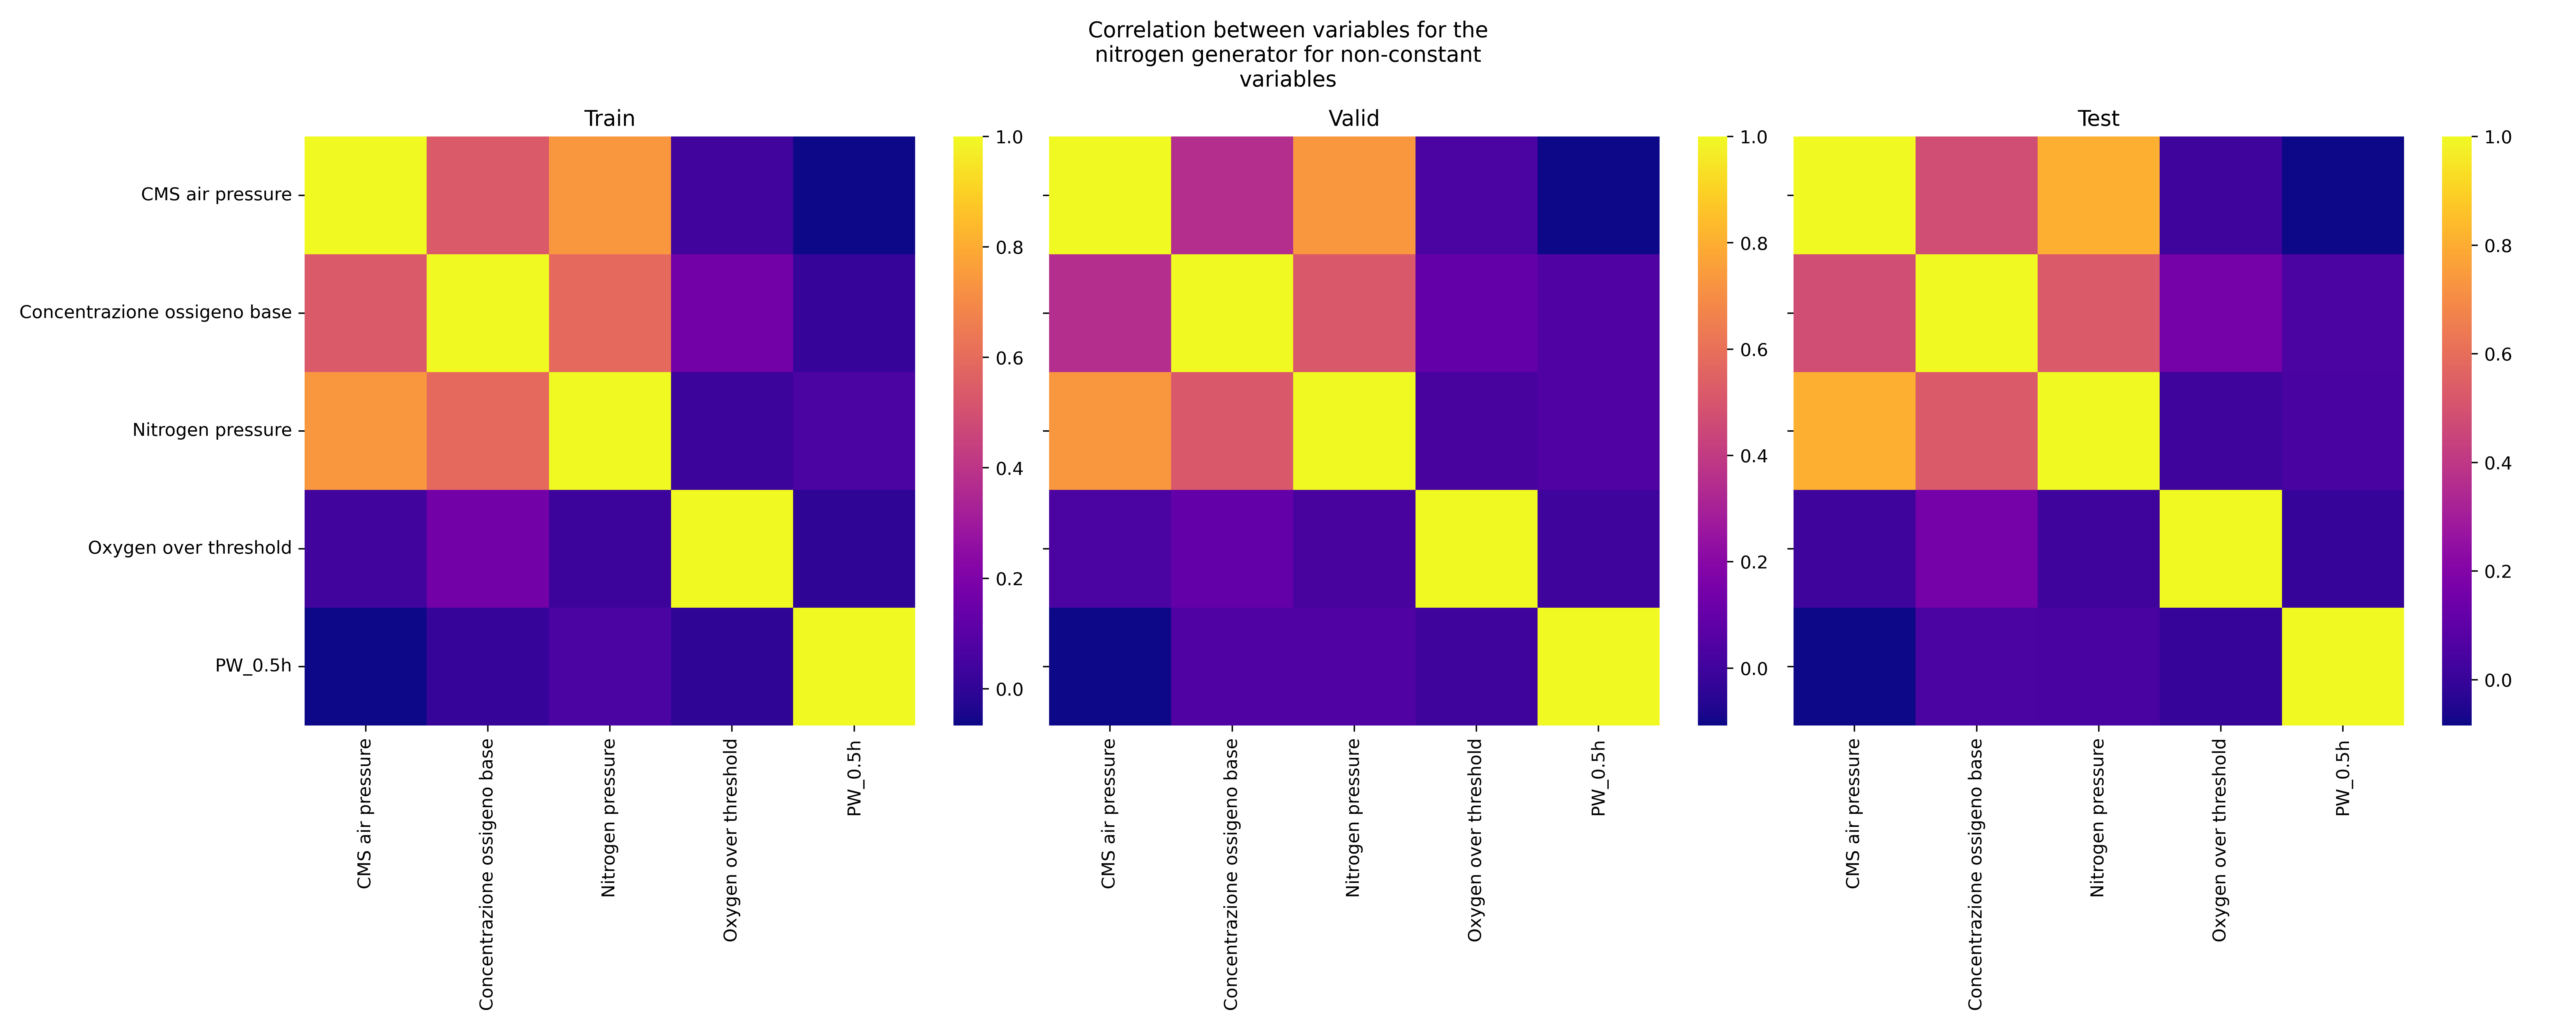
\includegraphics[width=16cm]{assets/test/nitrogen-generator/correlations.png}
    \caption{Correlation between variables in the nitrogen generator dataset splits. The label column is 'PW\_0.5h'.}
\end{figure}

Upon examination of the correlations, shown in figures 3 and 4, between variables for each dataset, there were no instances where any one variable
was significantly correlated with the target variable, 'PW\_0.5h'. We felt no need to drop additional features based
on these observations.

\paragraph{Feature Distributions}

\begin{figure}
    \centering
    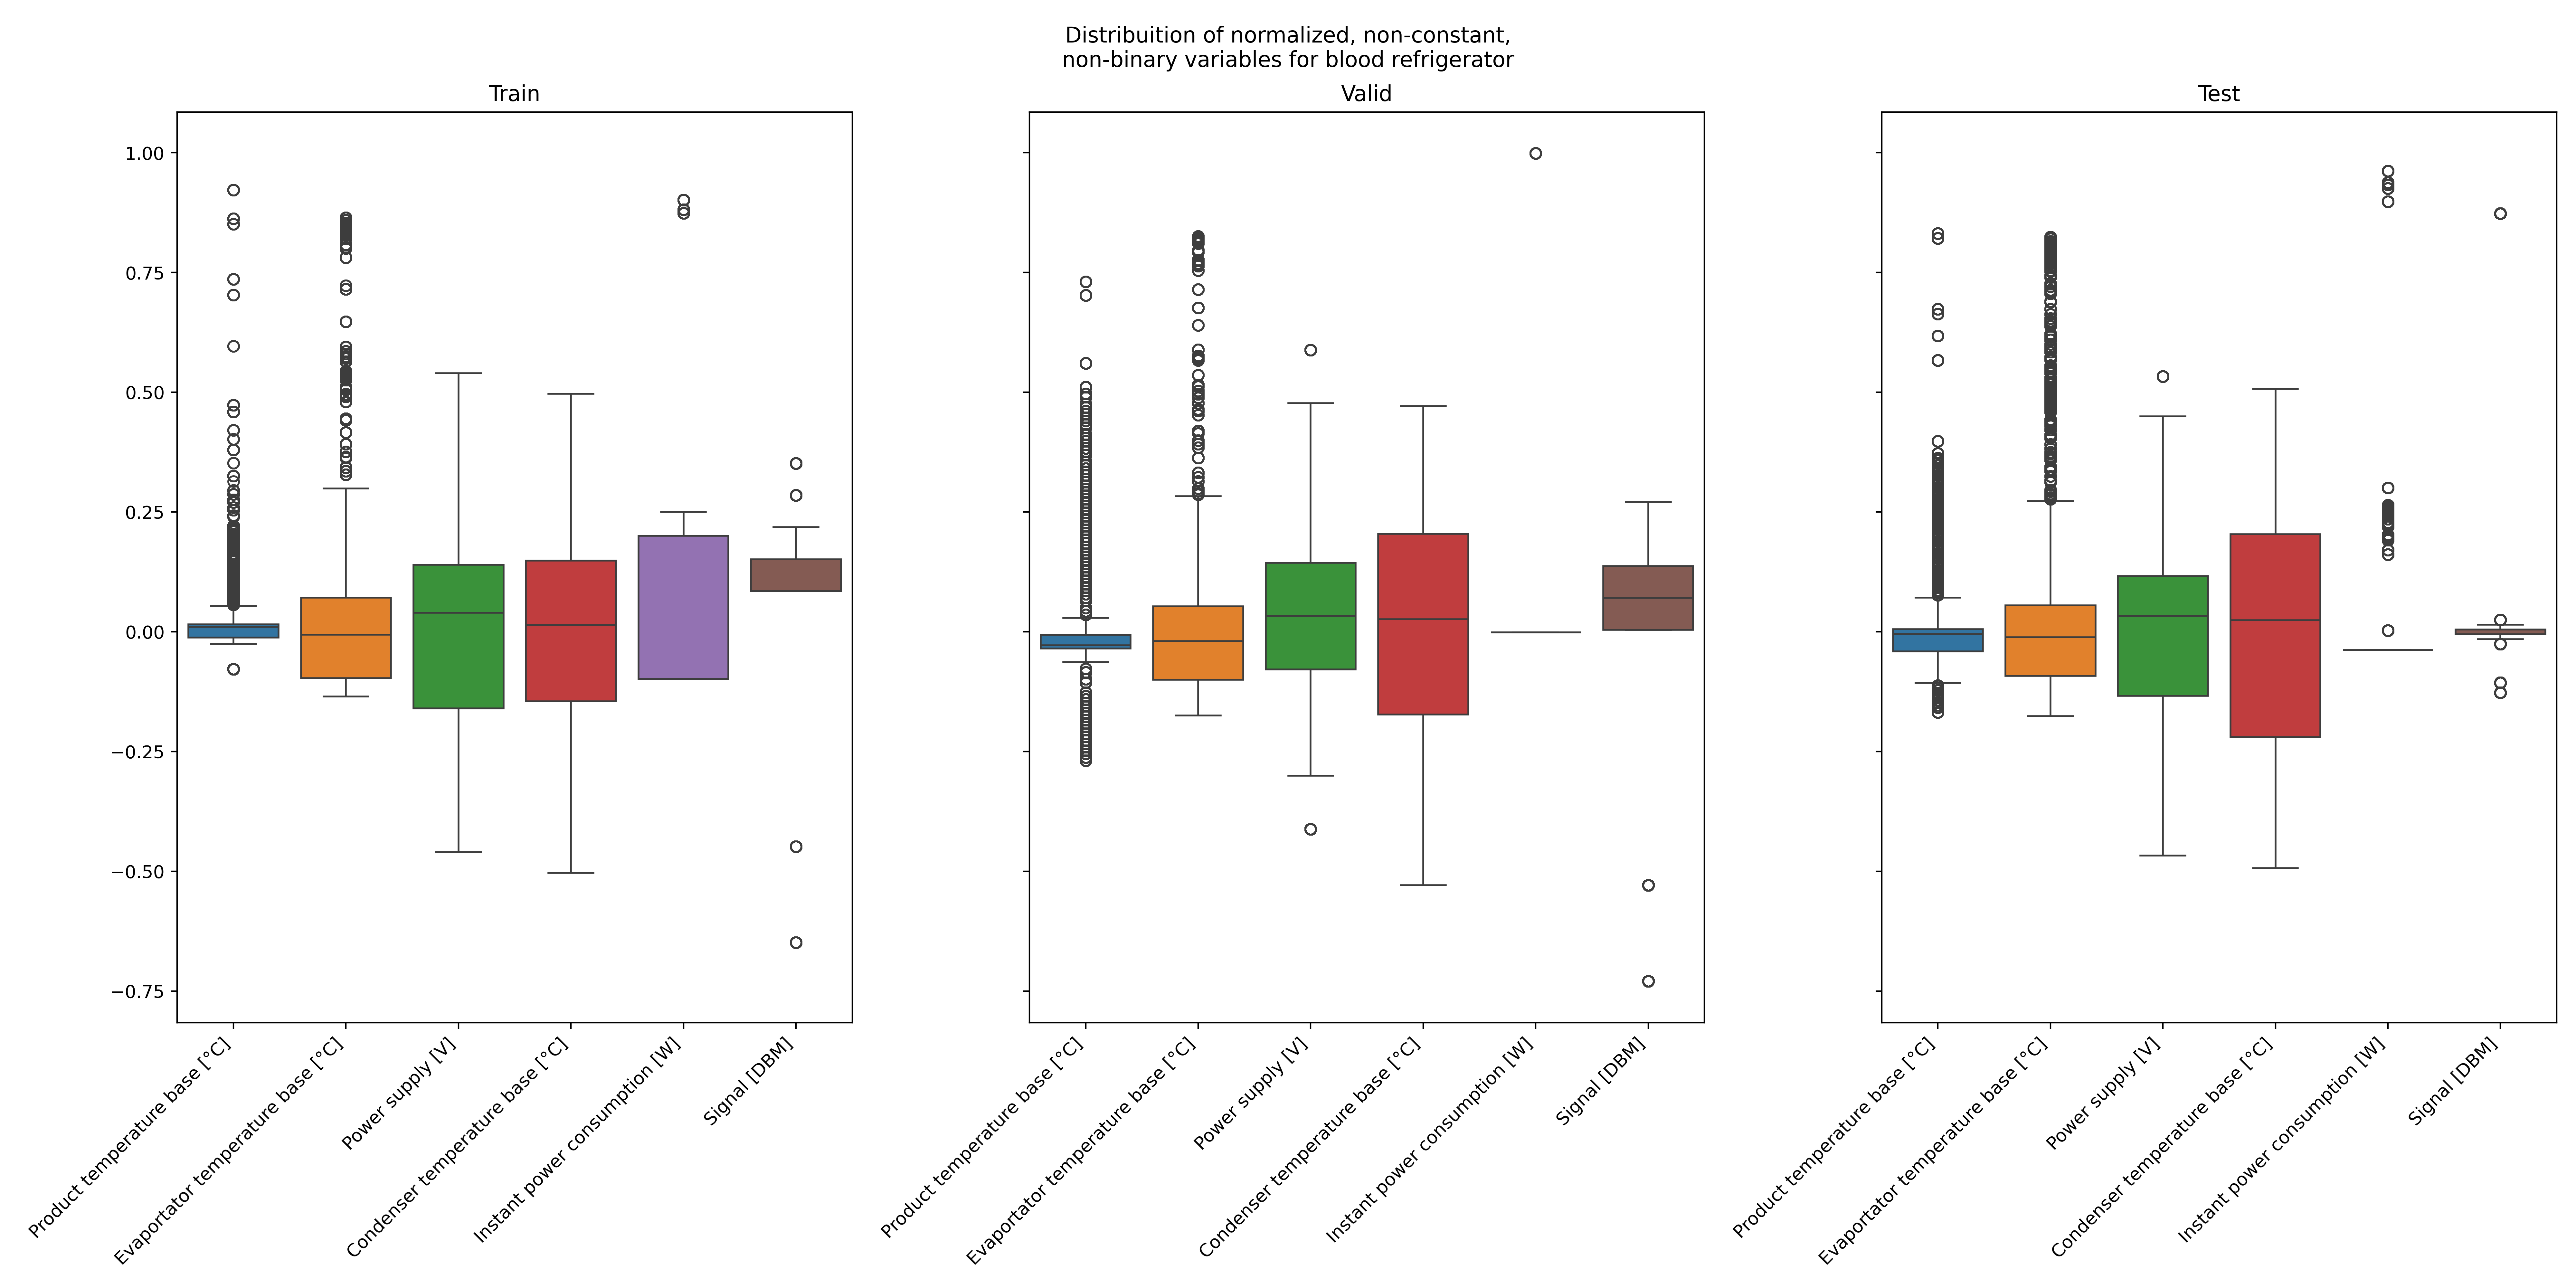
\includegraphics[height=7cm]{assets/test/blood-refrigerator/feature-distributions.png}
    \caption{Distribution of normalized, continuous variables for the blood refrigerator dataset splits.}
    \centering
    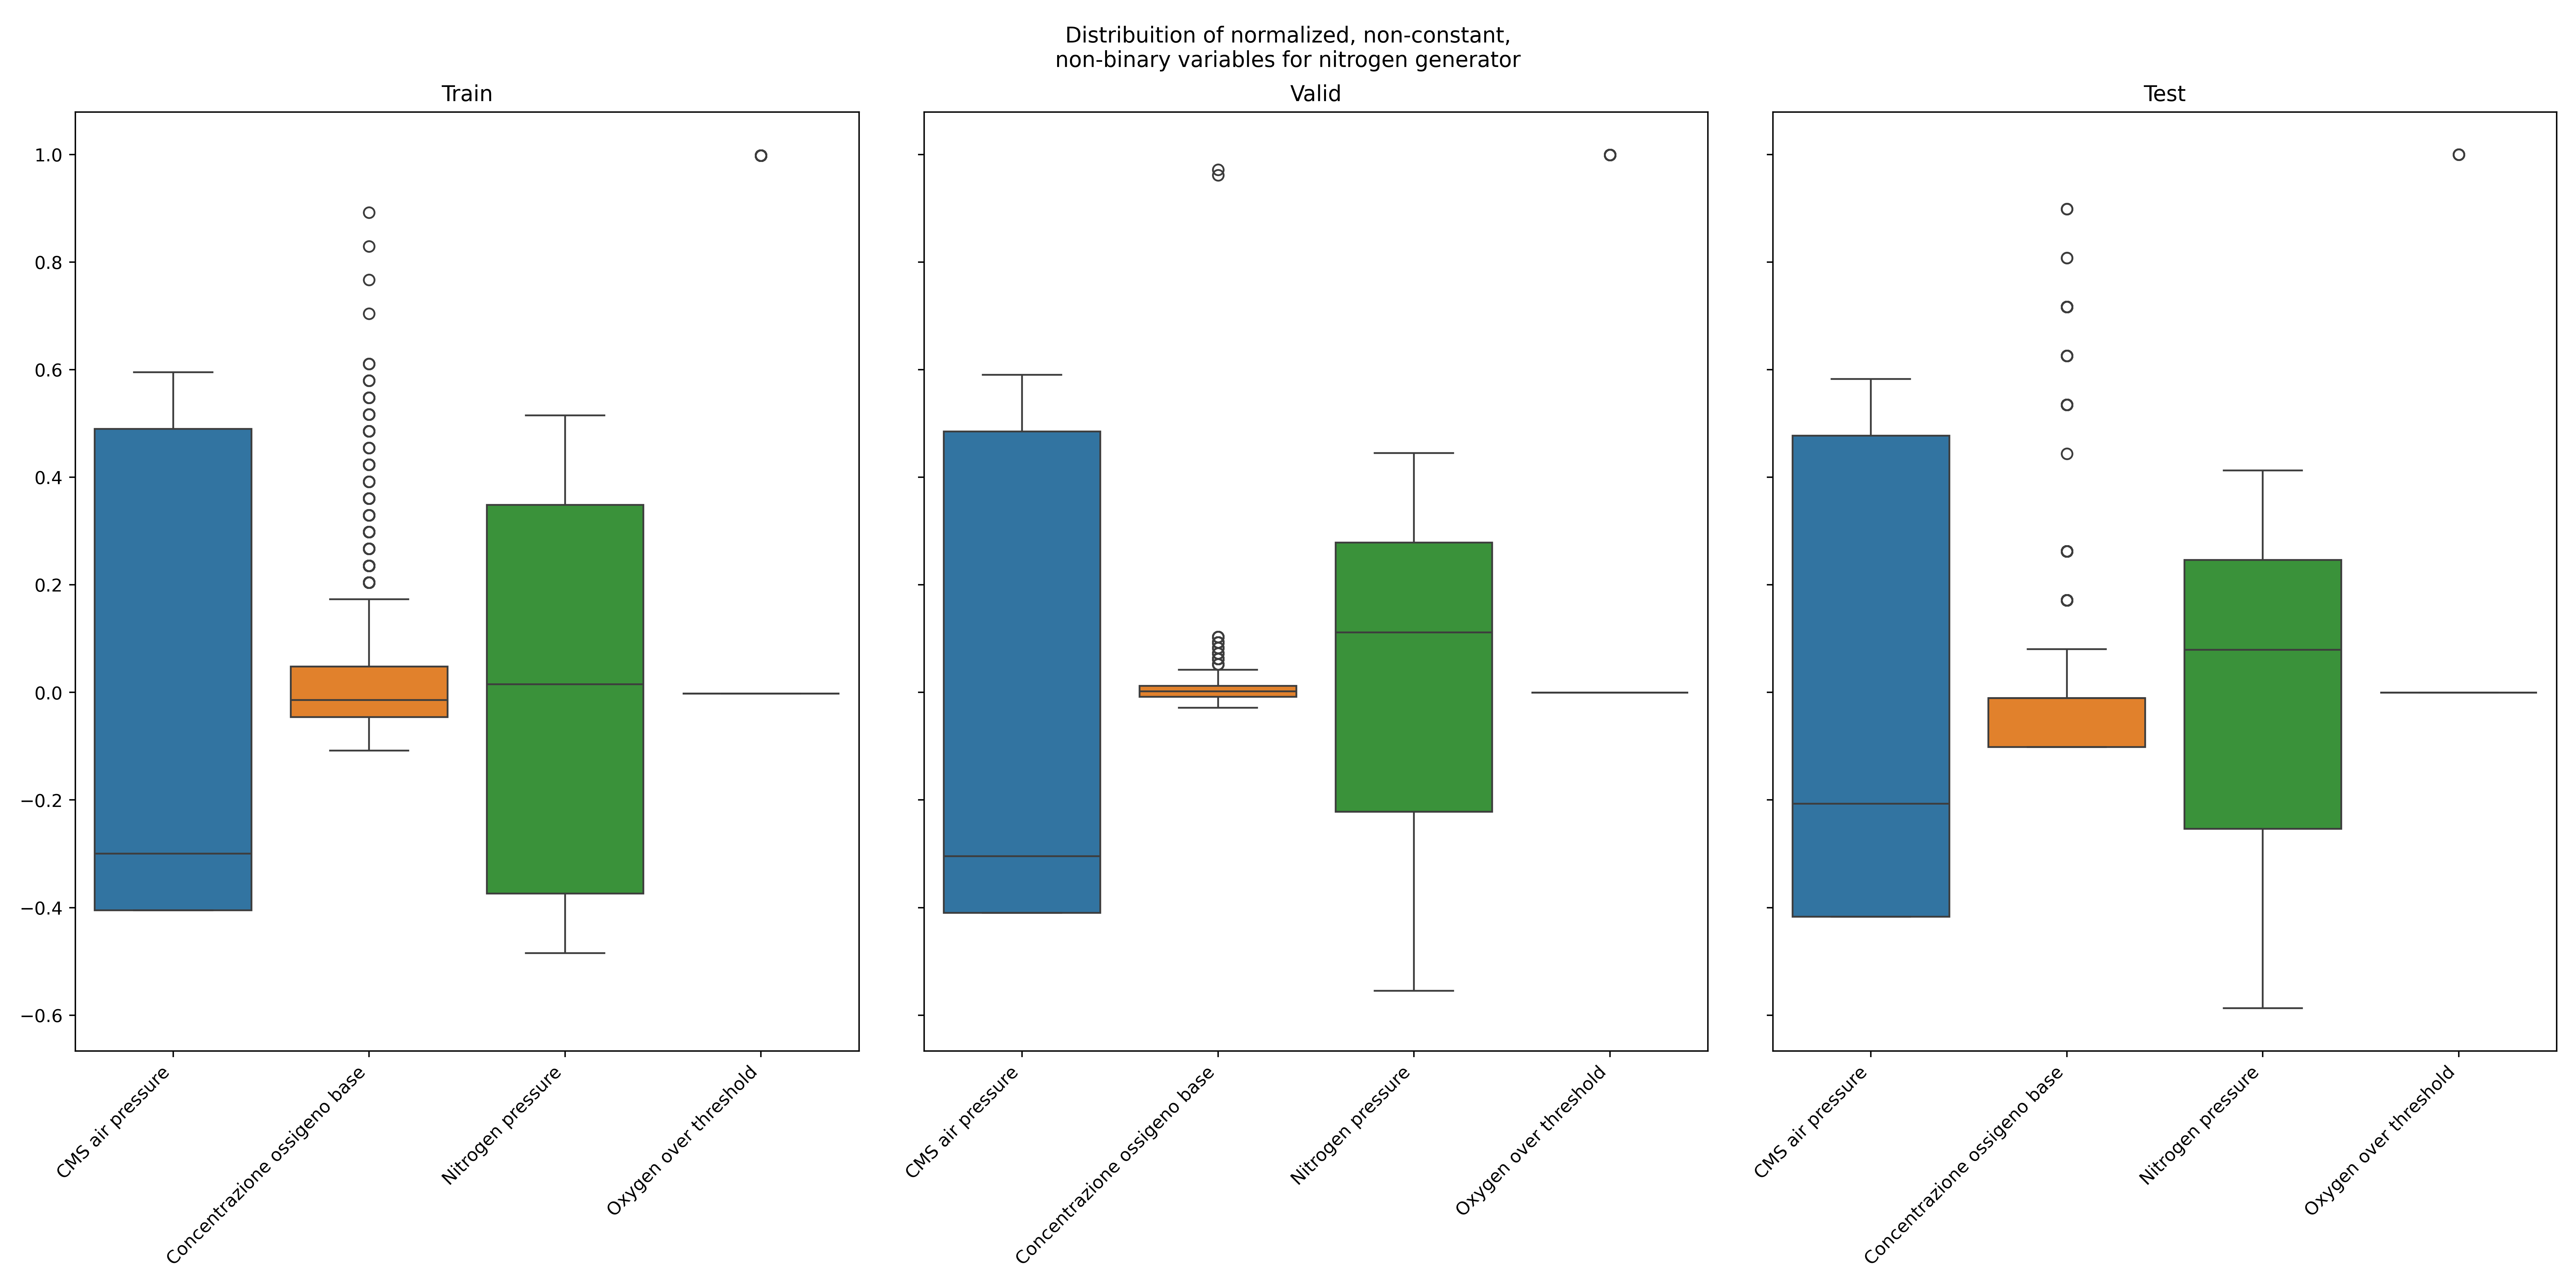
\includegraphics[height=7cm]{assets/test/nitrogen-generator/feature-distributions.png}
    \caption{Distribution of normalized, continuous variables for the nitrogen generator dataset splits.}
\end{figure}

Figures 5 and 6 show the distributions of the continuous variables for both machines. The blood refrigerator has, good representation
of most variables in the training set that appear in the validation and test splits.
 
For additional detailed discussion and analysis of the datasets, the reader is referred to \cite{pinciroli_vago_predicting_2024}.

\subsubsection{Processing}
Pre-processing of the data was kept fairly minimal. As mentioned above, we decided to drop any columns with zero variance as these
would not contribute any meaningful signal for any of our methods to learn from. This resulted in 12 columns for the blood refrigerator data
and 4 columns for the nitrogen generator data. The remaining continuous variables were normalized with:

\begin{equation}
    \hat{x_{it}}=\frac{x_{it}-\bar{x_{i}}}{\max{x_i}-\min{x_i}}
\end{equation}

for variable $i$ at time $t$.


\subsection{Models}
\subsubsection{T$^2$ Control Chart}
One method from SPC that is commonly used is the T$^{2}$-Control Chart with Upper Control Limit (UCL). Given a set of $n$
correlated characteristics $X_i$, assumed to follow a multivariate-normal distribution, the T$^{2}$
statistic is:

\begin{equation}
    T^{2} = m (\bar{x}-\mu)\Sigma^{-1}(\bar{x}-\mu)
\end{equation}

Where $m$ is the number of samples in the subgroup ($m=1$ is referred to as individual control charts),
$\bar{x}$ is the mean of a sample of $m$ vectors of measurements, $\Sigma$ is the covariance matrix (assuming it is known), and
$\mu$ is the in-control process mean (assuming it is known)\cite{lawson_introduction_2021}. For simplicity,
it should be assumed that all discussion is with regards to individual T$^2$-control charts unless otherwise
stated.

The UCL is $\chi^2$ distributed and is calculated at $\frac{\alpha}{2}$. In practice,

\begin{equation}
    \text{UCL}_{\frac{\alpha}{2}} = \frac{(k-1)^2}{k}f \left( 1-\frac{\alpha}{2};\frac{p}{2},\frac{(k-p-1)}{2}\right)
\end{equation}

where $f$ is the beta distribution. The Lower Control Limit (LCL)
is set to zero.

It is often the case that $\Sigma$ and $\mu$ are not known. These can be estimated from
the sample by:

\begin{equation}
    \mu \approx \hat{\mu} = \frac{1}{k} \sum_{i=1}^k \hat{x}_i
\end{equation}

where $\hat{x}_i$ are the observations from the in-control process sample, and

\begin{equation}
    \Sigma \approx \hat{\Sigma} = 
    \begin{bmatrix}
        \hat{\sigma}^2_{11} & \dots & \hat{\sigma}^2_{1n} \\
        \vdots & \ddots & \vdots \\
        \hat{\sigma}^2_{n1} & \dots & \hat{\sigma}^2_{nn}
    \end{bmatrix}
\end{equation}

where $\hat{\sigma}^2_{ij}$ is the variance between characteristics $X_i$ and $X_j$ from the 
in-control process sample.

To plot the $i^{th}$ point on the individual chart, $(1)$ becomes:

\begin{equation}
    T_i^{2} = (x_i-\hat{\mu})\hat{\Sigma}^{-1}(x_i-\hat{\mu})
\end{equation}

As new observations are made and new points added to the plot various signals may arise.
Perhaps the most apparent is a breach of the UCL (a new point with a T$^2$-statistic $>$ UCL).
This could suggest that something unusual happened with that single instance. There are many
other patterns that may arise. A continuous streak of 3-5 points beyond the 2 standard deviation
mark, 7 or more beyond 1 standard deviation, 8-9 points alternating sides of the center line in
a zig-zag pattern. All of these suggest different things about the underlying process and that
either the process should be investigated or a new in-control sample taken to establish
new charts.

We will be using the above technique largely as-is because it is a standard methodology and has
demonstrated itself to be very effective. We will use the last 25\%, 50\%, 75\%, and all
of the training data to establish the control parameters. This will allow us to evaluate the
effects of recency on the results. To determine when a "stop" signal should be raise, we have
defined two patterns that accept a variety of parameters. When the conditions specified by the
patterns are met, a 1 ("stop") is returned. Because this method is not trained in an iterative
manner, we do not train or evaluate using the validation time series.

During the experiments, we found that the performance when using the training data to construct
control charts for the test data yielded very poor results. So we included a set of results where
the control limits are set using the first 150 or 70 time steps for the blood refrigerator and nitrogen
generator, respectively, for each day in the test set. In other words, the control chart for a given day
would be determined based on the the sensor readings during the first part of its normal operation for a day.

The patterns we use are "n sequential breaches of the UCL or LCL" and "n total breaches of the UCL or LCL in a
window of length t". For the former case, if we raise a stop signal at the first instance of any window where all 
$n$ observations are above or below (including a mix of above and below) the control limits. For the latter, we 
raise a stop signal at the first instance of a window of $t$ time steps there are $n$ breaches above or below
the control limits.


\subsubsection{Transformer}

The transformer is an architecture with several components: a tokenizer, an embedding layer,
transformer layers, a task-specific head\cite{vaswani_attention_2023}. The transformer layer
is a collection of alternating multi-head attention layers and linear feed forward layers.
These models are often pre-trained on large collections of text as foundation models then
fine-tuned for specific tasks by adding a task-specific head that converts the representation
from the last hidden layer of the transformer body into a useable output. It is possible to
train transformers on more than just text. Many variations exist that operate on video, audio,
time series, and combinations of the above (multi-modal).

A family of open-source foundational time series transformer models was recently released\cite{goswami_moment_2024}
that has been pre-trained on a rich collection of time series data and can be fine-tuned for
specific tasks such as anomaly detection or classification. The models (MOMENT) were pre-trained
with univariate time series data with a variety of time horizons. When given multivariate
time series data, each variable is treated separately in its own channel.

The specific model we will be using has an architecture similar to the T5 encoder\cite{Raffel2019ExploringTL}
and has approximately 385MM parameters. We will be fine-tuning a freshly initialized linear
layer to perform the classification task.

For this model, we will extract rolling windows comprising 20 minutes (determined using the time stamps 
provided in the data) as the input sequence and the label for the time step immediately after the end of the
window as the target for learning. MOMENT requires all input sequences are 512 tokens in length, so
all inputs will be padded with zeros to meet the length requirement and masks will be generated
so the loss is calculated only from features related to the input sequence. We chose 20 minutes since
previous research found that was the window where the models typically performed best\cite{pinciroli_vago_predicting_2024}.

MOMENT will be fine tuned using the Adam optimizer\cite{Kingma2014AdamAM} with a learning rate of 0.001
that uses a cosine annealing schedule to a minimum of $10^{-6}$ for binary classification. Weight decay
is 0.1 and $\beta_1, \beta_2$ are 0.9 and 0.999, respectively. We use a batch size of 8. Fine-tuning is carried out over 5 epochs 
and the model is checkpointed at the end of each epoch if the validation loss decreased. Due to the high 
degree of class imbalance, we use normalized class weights in the loss function equal to:

\begin{equation}
    [w_0,w_1] = [1/p_0, 1/p_1] * (1/p_0+1/p_1)^{-1}
\end{equation}


\subsubsection{Reinforcement Learning}
Reinforcement learning is defined in the context of solving a Markov Decision Process (MDP). An MDP is a tuple
$(\mathcal{S},\mathcal{A},\mathcal{R},\mathbb{P})$ with a state space, action space, reward function, and
a probability to transition from state to state given an action. A state in the state space $s_i\in \mathcal{S}$
is a representation of the environment at time $i$. In our case, each $s$ is a vector in $\mathbb{R}^n$.
The action space is comprised only of {"Do nothing", "Stop"}, or, ${0,1}=\mathcal{A}$. Our reward function
is defined so that the agent receives a positive reward if it returns 0 while the label is still 0 or 1
when the label is 1. The agent will receive a negative reward if it returns a 1 when the label is 0 and
vice-versa. There is an additional penalty that is incurred for each time step that passes where the agent
has not stopped the machine (returned a 0) but the label is 1, specifically:

\[ \mathcal{R(s,a)} =
    \begin{cases}
        a=1 \land \text{PW\_0.5h}=1       &\to +1 \\
        a=1 \land \text{PW\_0.5h}=0       &\to -10 \\
        a=0 \land \text{PW\_0.5h}=1       &\to \sum_{i=0}^k i \text{ where $k$ is the time since the first stop signal} \\
        a=0 \land \text{PW\_0.5h}=0       &\to +0.01
    \end{cases}
\]

where PW\_0.5h$={0,1}$ indicates the label and $a$ the action chosen by the agent at that step. The transition probabilities
are defined by the temporal sequencing naturally present in the dataset and is deterministic in nature.

However, we observed extremely brittle policies by leaving the time series for each day in temporal order. So, we
shuffle all of the days during each episode to prevent the agent from trying to learn dependencies day-to-day. While
there is an argument to be made for the importance of day-to-day patterns, that is a problem that warrants its own
paper. For simplicity, we will proceed only trying to have the agents learn how to act within each day.

For both algorithms, the hidden dimension for the neural networks is determined by the number of input features for the machine.
PPO uses the first power of 2 larger than the input dimension and MCTS uses the second power of 2 larger than the input dimension.
These were determined empirically over a limited space. For the blood refrigerator, with 12 variables, the hidden layers of the
networks in the PPO agent have dimension 16 but dimension 32 for the MCTS agent. For the nitrogen generator the layers are 8 and
16, respectively.

\paragraph{Monte Carlo Tree Search}
The Monte Carlo Tree Search (MCTS) with neural guidance stores information in a tree structure with states as nodes
and actions connecting from that node to the next state that it transitioned to as a result of that action. It
gathers a number of paths by running simulations down the tree by selecting the action at each node that leads to
the node with the largest expected value, starting at the root, and propagating values back up
through the path based on a combination of the expected value for that state and the number of visits to that node
over the simulations. Some randomness is used to ensure some exploration can occur to increase the likelihood that
the algorithm will find the optimal policy.

The MCTS algorithm has 4 steps:
\begin{enumerate}
    \item Starting from the root, select child nodes until a leaf node is reached
    \item If the leaf node is not a state that is equal to the process being stopped, create child nodes for each
        possible action
    \item Perform a simulation by collecting paths from moving down the tree
    \item Pass the result from this simulation (rollout) up through all nodes in their respective paths
\end{enumerate}
Step 3 can be done randomly or with some sort of direction. This can be as simple as a greedy search (select the
child node with the largest reward) or can use a more complex method such as a neural network\cite{silver_mastering_2017,silver_mastering_2016}.
The neural network takes the position in the tree and returns a vector of probabilities to select each action
(the policy). These policy vectors are proportional to the exponential of the visit count for each node (i.e. 
$\pi\propto N(s,a)^{1/\tau}$, where $N$ is the visit count and $\tau$ a scaling value). The
neural network has two heads, one to return a policy and one to return a value for the node. Training is done
by minimizing the cross entropy loss between the policy and the actions yielding the highest reward, plus, the
mean squared error of the value of the current node and the discounted expectation of future returns. The ideal
situation is for the network to learn to correctly choose an action that will keep moving the agent towards
high-value states that yield, in aggregate, the largest cumulative reward.

We explored this method due to the unique nature of the policy optimization process and believed that it would
provide an interesting and challenging implementation.

The network is trained using the Adam optimizer\cite{Kingma2014AdamAM} with an initial learning rate of 0.0001
and uses cosine annealing to a minimum of $10^{-6}$. Weight decay is set to 0.01 and $\beta_1,\beta_2$ are 0.9
and 0.999, respectively. The discount factor for future rewards is $\gamma=0.99$. At the end of each time series
for a day, end of an episode, or every 4$^{th}$ time step, a "learning" process is triggered. The process begins
by collecting 100 simulations (paths) from the current tree using the current network. The agent samples
128 tuples from the 10,000 most recent experiences $\left(s_t, a_t, r_t, s_{t+1}\right)$ to train the network. Each epoch
is considered complete when the agent has progressed through all of the days' time series in the training set.
We train the agent for 30 epochs and use early stopping if there is no improvement in the mean reward on the
validation set after 5 epochs.

\paragraph{Proximal Policy Optimization}
The proximal policy optimization (PPO)\cite{Schulman2017ProximalPO} is an extention of their earlier trust-region policy
optimization algorithm\cite{Schulman2015TrustRP}. It is an on policy algorithm and uses two neural networks during training. 
The agent uses both a neural network to learn a policy, that is sampled
from using a categorical distribution, to determine what action to take in a given state and a separate network to learn
the expected value of a given state. We sample from a distribuition determined by the policy to allow some amount of exploration
to persist during training. This can help reduce the likelihood an agent gets stuck in a locally optimal policy and unable to 
find the globally optimal policy. The policy updates are clipped to prevent any single update from being too large and destabilizing
the learning process.

The PPO algorithm contains some simplifications and improves the sample
efficiency by using multiple policy updates per episode (or epoch). During each episode, the policy and value networks are
updated $k$ times, each time using a different minibatch of recent experiences stored in the agent's memory. A simple queue
is used to store the experiences in the order they occur up to a total of 10,000 experiences. As new ones are added the oldest
experiences will be removed from the memory to maintain 10,000 examples. We use 10 updates per learning instance with an
experience replay batch size of 64 per update. The $\epsilon-$clipping parameter is set to 0.2 (taken from the paper) and a
learning rate of 0.0003 is used with the Adam\cite{Kingma2014AdamAM} optimizer. The reward discounting factor is set to 0.999.

We chose to explore this algorithm since it has demonstrated excellent performance in a variety of continuous state spaces and
is likely to demonstrate better convergence in this scenario. While the MCTS algorithm is very powerful, it tends to perform best
when used either when there is an opponent the agent is playing against and/or when the state space is discrete.

\subsection{Evaluation}
The trained model or agent is used to generate predictions on the held-out test set. We collect the recall, precision, and 
F$_1$ (in both strict and relaxed settings) as well as the mean-time-from-event (MTFE). The MTFE measures the mean mistiming
of the method, mathematically:

\begin{equation}
    MTFE = \frac{1}{K}\sum_k (t_km-t_ke)
\end{equation}

The strict version of the classification metrics is determined where the model or agent returns the stop signal only on the
very first occurence of the stop signal in that time series or, in the case where a time series does not stop, if the agent
never raises the stop signal. The relaxed variation considers any stop signal returned by the model at any stop label
in the time series as correct.

The precision, recall, and F$_1$ are calculated in the usual manner. The only difference arises in the use of strict or 
lenient evaluation protocols.

Each method is trained on the training split then evaluated on the held-out test split. The control chart and transformer
return predictions for each time step while the RL agents stop making predictions for a given day until they return a stop
action or reached the end of the day's time series. The predictions are calculated on a per-day basis for each test split (
e.g. the 27 days for the blood refrigerator test set are each given a single prediction).


\section{Results}

\subsection{T$^2$ Control Charts}

\subsubsection{Blood Refrigerator}

Tables 2-5 report the MTFE, F1, Precision, and Recall scores for the T$^2$ control charts that were determined based on the
last $p$ proportion of the training split. Table 6 includes the same metrics but in the case where the first 150 time steps
were used to determine the control chart parameters for the day. The patterns are described in the first column of each table
and translate to "XperYat$\alpha$" or "XseqAt$\alpha$" where $\alpha=0.05$, X is the number of breaches, and Y is the length
of the window.

Overall, there are not many differences between the results for the lenient and strict evaluation protocols for all tables.
The approximate spacing between time intervals is 34 seconds. The values that most closely mimic the 20 minute RW with 30
minute PW would be the "20per40at0.05" and "40seqAt0.05" rows from each table.

\begin{table}[h]
    \begin{tabular}{|c|cc|cc|cc|cc|}
        \hline \\
        \textbf{}       & \multicolumn{8}{c|}{Proportion of Training Split}                                                                                                        \\
                        & \multicolumn{2}{c}{0.25}            & \multicolumn{2}{c}{0.50}            & \multicolumn{2}{c}{0.75}            & \multicolumn{2}{c|}{1.00}              \\ 
                        & \multicolumn{1}{c}{Lenient} & \multicolumn{1}{c}{Strict} & \multicolumn{1}{c}{Lenient} & \multicolumn{1}{c}{Strict} & \multicolumn{1}{c}{Lenient} & \multicolumn{1}{c}{Strict} & \multicolumn{1}{c}{Lenient} & \multicolumn{1}{c|}{Strict} \\ \hline
        5per10at0.05    & -328          & -328          & -249          & -249          & -421          & -421          & -422           & -422           \\
        10per20at0.05   & -398          & -398          & -243          & -243          & -422          & -422          & -422           & -422           \\
        20per40at0.05   & -400          & -400          & -232          & -232          & -422          & -422          & -422           & -422           \\
        30per60at0.05   & -400          & -400          & -213          & -213          & -422          & -422          & -422           & -422           \\
        40per80at0.05   & -400          & -400          & -185          & -185          & -422          & -422          & -422           & -422           \\
        60per120at0.05  & -391          & -391          & -192          & -192          & -422          & -422          & -422           & -422           \\
        120per240at0.05 & -365          & -365          & -110          & -110          & -422          & -422          & -422           & -422           \\ \hline
        5seqAt0.05      & -326          & -326          & -245          & -245          & -421          & -421          & -421           & -421           \\ 
        10seqAt0.05     & -392          & -392          & -177          & -177          & -421          & -421          & -421           & -421           \\
        20seqAt0.05     & -343          & -343          & \textbf{9}    & \textbf{9}    & -421          & -421          & -418           & -418           \\
        30seqAt0.05     & -316          & -316          & 197           & 198           & -397          & -397          & -383           & -383           \\
        40seqAt0.05     & -299          & -299          & 107           & 110           & -397          & -397          & -383           & -383           \\
        60seqAt0.05     & -305          & -305          & 188           & 193           & -377          & -377          & \textit{-236*} & \textit{-234*} \\
        120seqAt0.05    & \textbf{-284} & \textbf{-284} & \textit{-27*} & \textit{-22*} & \textbf{-298} & \textbf{-298} & \textbf{34}    & \textbf{42}    \\ \hline
        \textbf{Mean}   & \textbf{-353} & \textbf{-353} & \textbf{-98}  & \textbf{-97}  & \textbf{-406} & \textbf{-406} & \textbf{-370}  & \textbf{-369}  \\ \hline
    \end{tabular}
    \caption{Mean Time From Event for the T$^2$ Control Charts trained on varying portions of the training split. Best absolute result per column in bold, best without surpasing the start of failure in italics with *}
\end{table}

\begin{table}[]
    \begin{tabular}{|c|cc|cc|cc|cc|}
        \hline
        \textbf{}       & \multicolumn{8}{c|}{Proportion of Training Split}                                                                                                                                                                                          \\
                        & \multicolumn{2}{c}{0.25}                                 & \multicolumn{2}{c}{0.50}                                 & \multicolumn{2}{c}{0.75}                                 & \multicolumn{2}{c|}{1.00}                                 \\
                        & \multicolumn{1}{c}{Lenient} & \multicolumn{1}{c}{Strict} & \multicolumn{1}{c}{Lenient} & \multicolumn{1}{c}{Strict} & \multicolumn{1}{c}{Lenient} & \multicolumn{1}{c}{Strict} & \multicolumn{1}{c}{Lenient} & \multicolumn{1}{c|}{Strict} \\ \hline
        5per10at0.05    & 0.00                        & 0.00                       & 0.20                        & 0.20                       & 0.00                        & 0.00                       & 0.00                        & 0.00                       \\
        10per20at0.05   & 0.11                        & 0.11                       & 0.29                        & 0.29                       & 0.00                        & 0.00                       & 0.00                        & 0.00                       \\
        20per40at0.05   & 0.11                        & 0.11                       & 0.29                        & 0.29                       & 0.00                        & 0.00                       & 0.00                        & 0.00                       \\
        30per60at0.05   & 0.11                        & 0.11                       & 0.36                        & 0.36                       & 0.00                        & 0.00                       & 0.00                        & 0.00                       \\
        40per80at0.05   & 0.11                        & 0.11                       & 0.36                        & 0.36                       & 0.00                        & 0.00                       & 0.00                        & 0.00                       \\
        60per120at0.05  & 0.11                        & 0.11                       & 0.36                        & 0.36                       & 0.00                        & 0.00                       & 0.00                        & 0.00                       \\
        120per240at0.05 & 0.11                        & 0.11                       & 0.36                        & 0.36                       & 0.00                        & 0.00                       & 0.00                        & 0.00                       \\ \hline
        5seqAt0.05      & 0.00                        & 0.00                       & 0.20                        & 0.20                       & 0.00                        & 0.00                       & 0.00                        & 0.00                       \\ 
        10seqAt0.05     & 0.11                        & 0.11                       & 0.29                        & 0.29                       & 0.00                        & 0.00                       & 0.00                        & 0.00                       \\
        20seqAt0.05     & 0.11                        & 0.11                       & 0.36                        & 0.36                       & 0.00                        & 0.00                       & 0.00                        & 0.00                       \\
        30seqAt0.05     & 0.11                        & 0.11                       & 0.48                        & 0.42                       & 0.00                        & 0.00                       & 0.00                        & 0.00                       \\
        40seqAt0.05     & 0.11                        & 0.11                       & 0.59                        & 0.54                       & 0.00                        & 0.00                       & 0.00                        & 0.00                       \\
        60seqAt0.05     & 0.20                        & 0.20                       & 0.67                        & 0.62                       & 0.00                        & 0.00                       & 0.11                        & 0.11                       \\
        120seqAt0.05    & \textbf{0.29}               & \textbf{0.29}              & \textbf{0.82}               & \textbf{0.79}              & \textbf{0.10}               & \textbf{0.10}              & \textbf{0.27}               & \textbf{0.27}              \\ \hline
        \textbf{Mean}   & \textbf{0.11}               & \textbf{0.11}              & \textbf{0.40}               & \textbf{0.39}              & \textbf{0.01}               & \textbf{0.01}              & \textbf{0.03}               & \textbf{0.03}              \\ \hline
    \end{tabular}
    \caption{F$_1$ scores for T$^2$ Control Charts on varying portions of the training split. Best in bold.}
\end{table}
 
\begin{table}[]
    \begin{tabular}{|c|cc|cc|cc|cc|}
        \hline
        \textbf{}       & \multicolumn{8}{c|}{Proportion of Training Split}                                                                                                                                                                                          \\
                        & \multicolumn{2}{c}{0.25}                                 & \multicolumn{2}{c}{0.50}                                 & \multicolumn{2}{c}{0.75}                                 & \multicolumn{2}{c|}{1.00}                                 \\
                        & \multicolumn{1}{c}{Lenient} & \multicolumn{1}{c}{Strict} & \multicolumn{1}{c}{Lenient} & \multicolumn{1}{c}{Strict} & \multicolumn{1}{c}{Lenient} & \multicolumn{1}{c}{Strict} & \multicolumn{1}{c}{Lenient} & \multicolumn{1}{c|}{Strict} \\ \hline
        5per10at0.05    & 0                           & 0                          & 1                           & 1                          & 0                           & 0                          & 0                           & 0                          \\
        10per20at0.05   & 1                           & 1                          & 1                           & 1                          & 0                           & 0                          & 0                           & 0                          \\
        20per40at0.05   & 1                           & 1                          & 1                           & 1                          & 0                           & 0                          & 0                           & 0                          \\
        30per60at0.05   & 1                           & 1                          & 1                           & 1                          & 0                           & 0                          & 0                           & 0                          \\
        40per80at0.05   & 1                           & 1                          & 1                           & 1                          & 0                           & 0                          & 0                           & 0                          \\
        60per120at0.05  & 1                           & 1                          & 1                           & 1                          & 0                           & 0                          & 0                           & 0                          \\
        120per240at0.05 & 1                           & 1                          & 1                           & 1                          & 0                           & 0                          & 0                           & 0                          \\ \hline
        5seqAt0.05      & 0                           & 0                          & 1                           & 1                          & 0                           & 0                          & 0                           & 0                          \\
        10seqAt0.05     & 1                           & 1                          & 1                           & 1                          & 0                           & 0                          & 0                           & 0                          \\
        20seqAt0.05     & 1                           & 1                          & 1                           & 1                          & 0                           & 0                          & 0                           & 0                          \\
        30seqAt0.05     & 1                           & 1                          & 1                           & 1                          & 0                           & 0                          & 0                           & 0                          \\
        40seqAt0.05     & 1                           & 1                          & 1                           & 1                          & 0                           & 0                          & 0                           & 0                          \\
        60seqAt0.05     & 1                           & 1                          & 1                           & 1                          & 0                           & 0                          & 1                           & 1                          \\
        120seqAt0.05    & 1                           & 1                          & 1                           & 1                          & 1                           & 1                          & 1                           & 1                          \\ \hline
        \textbf{Mean}   & \textbf{0.86}               & \textbf{0.86}              & \textbf{1.00}               & \textbf{1.00}              & \textbf{0.07}               & \textbf{0.07}              & \textbf{0.14}               & \textbf{0.14}             \\ \hline
    \end{tabular}
    \caption{Precision scores. Best in bold.}
\end{table}

\begin{table}[]
    \begin{tabular}{|c|cc|cc|cc|cc|}
        \hline
        \textbf{}       & \multicolumn{8}{c|}{Proportion of Training Split}                                                                                                                                                                                          \\
                        & \multicolumn{2}{c}{0.25}                                 & \multicolumn{2}{c}{0.50}                                 & \multicolumn{2}{c}{0.75}                                 & \multicolumn{2}{c|}{1.00}                                 \\
                        & \multicolumn{1}{c}{Lenient} & \multicolumn{1}{c}{Strict} & \multicolumn{1}{c}{Lenient} & \multicolumn{1}{c}{Strict} & \multicolumn{1}{c}{Lenient} & \multicolumn{1}{c}{Strict} & \multicolumn{1}{c}{Lenient} & \multicolumn{1}{c|}{Strict} \\ \hline
        5per10at0.05    & 0.00                        & 0.00                       & 0.11                        & 0.11                       & 0.00                        & 0.00                       & 0.00                        & 0.00                       \\
        10per20at0.05   & 0.06                        & 0.06                       & 0.17                        & 0.17                       & 0.00                        & 0.00                       & 0.00                        & 0.00                       \\
        20per40at0.05   & 0.06                        & 0.06                       & 0.17                        & 0.17                       & 0.00                        & 0.00                       & 0.00                        & 0.00                       \\
        30per60at0.05   & 0.06                        & 0.06                       & 0.22                        & 0.22                       & 0.00                        & 0.00                       & 0.00                        & 0.00                       \\
        40per80at0.05   & 0.06                        & 0.06                       & 0.22                        & 0.22                       & 0.00                        & 0.00                       & 0.00                        & 0.00                       \\
        60per120at0.05  & 0.06                        & 0.06                       & 0.22                        & 0.22                       & 0.00                        & 0.00                       & 0.00                        & 0.00                       \\
        120per240at0.05 & 0.06                        & 0.06                       & 0.22                        & 0.22                       & 0.00                        & 0.00                       & 0.00                        & 0.00                       \\ \hline
        5seqAt0.05      & 0.00                        & 0.00                       & 0.11                        & 0.11                       & 0.00                        & 0.00                       & 0.00                        & 0.00                       \\
        10seqAt0.05     & 0.06                        & 0.06                       & 0.17                        & 0.17                       & 0.00                        & 0.00                       & 0.00                        & 0.00                       \\
        20seqAt0.05     & 0.06                        & 0.06                       & 0.22                        & 0.22                       & 0.00                        & 0.00                       & 0.00                        & 0.00                       \\
        30seqAt0.05     & 0.06                        & 0.06                       & 0.32                        & 0.26                       & 0.00                        & 0.00                       & 0.00                        & 0.00                       \\
        40seqAt0.05     & 0.06                        & 0.06                       & 0.42                        & 0.37                       & 0.00                        & 0.00                       & 0.00                        & 0.00                       \\
        60seqAt0.05     & 0.11                        & 0.11                       & 0.50                        & 0.45                       & 0.00                        & 0.00                       & 0.06                        & 0.06                       \\
        120seqAt0.05    & \textbf{0.17}               & \textbf{0.17}              & \textbf{0.70}               & \textbf{0.65}              & \textbf{0.05}               & \textbf{0.05}              & \textbf{0.16}               & \textbf{0.16}              \\ \hline
    \end{tabular}
    \caption{Recall scores. Best in bold.}
\end{table}

Across all of tables 2-5, the best results are when only the most recent 50\% of the training split is used to determine the
charts. The weakest results are when 75\% of the training split is used. It also tends to be the case that a higher number of
breaches per window produces stronger results.

\begin{table}[]
    \begin{tabular}{|cc|cccc|}
        \hline
                                         &         & Mean Time From Event & Precision & Recall        & F1            \\ \hline
        \multirow{2}{*}{5per10at0.05}    & Lenient & -421.37              & 1.00      & 0.74          & 0.85          \\
                                         & Strict  & -421.37              & 1.00      & 0.74          & 0.85          \\ \hline
        \multirow{2}{*}{10per20at0.05}   & Lenient & -420.52              & 1.00      & 0.74          & 0.85          \\
                                         & Strict  & -420.52              & 1.00      & 0.74          & 0.85          \\ \hline
        \multirow{2}{*}{20per40at0.05}   & Lenient & -410.81              & 1.00      & 0.74          & 0.85          \\
                                         & Strict  & -410.81              & 1.00      & 0.74          & 0.85          \\ \hline
        \multirow{2}{*}{30per60at0.05}   & Lenient & -413.67              & 1.00      & 0.74          & 0.85          \\
                                         & Strict  & -413.67              & 1.00      & 0.74          & 0.85          \\ \hline
        \multirow{2}{*}{40per80at0.05}   & Lenient & -402.89              & 1.00      & 0.74          & 0.85          \\
                                         & Strict  & -402.89              & 1.00      & 0.74          & 0.85          \\ \hline
        \multirow{2}{*}{60per120at0.05}  & Lenient & -402.11              & 1.00      & 0.74          & 0.85          \\
                                         & Strict  & -402.11              & 1.00      & 0.74          & 0.85          \\ \hline
        \multirow{2}{*}{120per240at0.05} & Lenient & \textbf{-377.67}     & 1.00      & 0.74          & 0.85          \\
                                         & Strict  & \textbf{-377.67}     & 1.00      & 0.74          & 0.85          \\ \hline
        \multirow{2}{*}{5seqAt0.05}      & Lenient & -421.19              & 1.00      & 0.74          & 0.85          \\
                                         & Strict  & -421.19              & 1.00      & 0.74          & 0.85          \\ \hline
        \multirow{2}{*}{10seqAt0.05}     & Lenient & -419.74              & 1.00      & 0.74          & 0.85          \\
                                         & Strict  & -419.74              & 1.00      & 0.74          & 0.85          \\ \hline
        \multirow{2}{*}{20seqAt0.05}     & Lenient & -393.89              & 1.00      & 0.74          & 0.85          \\
                                         & Strict  & -393.89              & 1.00      & 0.74          & 0.85          \\ \hline
        \multirow{2}{*}{30seqAt0.05}     & Lenient & -380.89              & 1.00      & 0.74          & 0.85          \\
                                         & Strict  & -380.89              & 1.00      & 0.74          & 0.85          \\ \hline
        \multirow{2}{*}{40seqAt0.05}     & Lenient & -392.04              & 1.00      & 0.74          & 0.85          \\
                                         & Strict  & -392.04              & 1.00      & 0.74          & 0.85          \\ \hline
        \multirow{2}{*}{60seqAt0.05}     & Lenient & -417.85              & 1.00      & 0.79          & 0.88          \\
                                         & Strict  & -417.85              & 1.00      & 0.79          & 0.88          \\ \hline
        \multirow{2}{*}{120seqAt0.05}    & Lenient & -421.52              & 1.00      & \textbf{0.84} & \textbf{0.91} \\
                                         & Strict  & -421.52              & 1.00      & \textbf{0.84} & \textbf{0.91} \\ \hline
    \end{tabular}
    \caption{Results when using the first 150 time steps of each day. Best for each metric in bold.}
\end{table}

\clearpage
\subsubsection{Nitrogen Generator}

Tables 7 and 8 report the MTFE, F1, Precision, and Recall scores for the T$^2$ control charts that were determined based on the
last $p$ proportion of the training split. The precision, recall, and F$_1$ results were identical for all patterns and all splits
so the results in table 8 represent all of those metrics. During the experiments to use the first portion of the day, we were unable
to find an interval of time that would result in an invertible covariance matrix, thus the statistics could not be computed.
The patterns are described in the first column of each table
and translate to "XperYat$\alpha$" or "XseqAt$\alpha$" where $\alpha=0.05$, X is the number of breaches, and Y is the length
of the window.

Overall, there are not many differences between the results for the lenient and strict evaluation protocols for all tables.
The approximate spacing between time intervals is 1 minute. The values that most closely mimic the 20 minute RW with 30
minute PW would be the "30seqAt0.05" row from each table.

\begin{table}[h!]
    \begin{tabular}{|c|cc|cc|cc|cc|}
        \hline
                        & \multicolumn{8}{c|}{Proportion of Training Split}                                                                              \\
                        & \multicolumn{2}{c}{0.25}      & \multicolumn{2}{c}{0.5}       & \multicolumn{2}{c}{0.75}      & \multicolumn{2}{c|}{1}         \\
                        & \multicolumn{1}{c}{Lenient} & \multicolumn{1}{c}{Strict} & \multicolumn{1}{c}{Lenient} & \multicolumn{1}{c}{Strict} & \multicolumn{1}{c}{Lenient} & \multicolumn{1}{c}{Strict} & \multicolumn{1}{c}{Lenient} & \multicolumn{1}{c|}{Strict} \\ \hline
        5per10at0.05    & -764          & -764          & -764          & -764          & -791          & -791          & -791          & -791          \\
        10per20at0.05   & -755          & -755          & -764          & -764          & -791          & -791          & -791          & -791          \\
        20per40at0.05   & -757          & -757          & -763          & -763          & -791          & -791          & -791          & -791          \\
        30per60at0.05   & -758          & -758          & -765          & -765          & -791          & -791          & -791          & -791          \\
        40per80at0.05   & -756          & -756          & -766          & -766          & -791          & -791          & -791          & -791          \\
        60per120at0.05  & -683          & -683          & -767          & -767          & -791          & -791          & -791          & -791          \\
        120per240at0.05 & -691          & -691          & -691          & -691          & -791          & -791          & -791          & -791          \\ \hline
        5seqAt0.05      & -755          & -755          & -762          & -762          & -791          & -791          & -791          & -791          \\
        10seqAt0.05     & -753          & -753          & -762          & -762          & -791          & -791          & -791          & -791          \\
        20seqAt0.05     & \textbf{-676} & \textbf{-676} & -759          & -759          & -791          & -791          & -791          & -791          \\
        30seqAt0.05     & \textbf{-676} & \textbf{-676} & -759          & -759          & -791          & -791          & -791          & -791          \\
        40seqAt0.05     & \textbf{-676} & \textbf{-676} & \textbf{-676} & \textbf{-676} & -791          & -791          & -791          & -791          \\
        60seqAt0.05     & \textbf{-676} & \textbf{-676} & \textbf{-676} & \textbf{-676} & -791          & -791          & -791          & -791          \\
        120seqAt0.05    & \textbf{-676} & \textbf{-676} & \textbf{-676} & \textbf{-676} & -791          & -791          & -791          & -791          \\ \hline
        \textbf{Mean}   & \textbf{-718} & \textbf{-718} & \textbf{-739} & \textbf{-739} & \textbf{-791} & \textbf{-791} & \textbf{-791} & \textbf{-791} \\ \hline
    \end{tabular}
    \caption{Mean Time From Event for the T$^2$ Control Charts trained on varying portions of the training split. Best absolute result per column in bold, best without surpasing the start of failure in italics with *}
\end{table}

\begin{table}[]
    \begin{tabular}{|c|cc|cc|cc|cc|}
        \hline
                        & \multicolumn{8}{c|}{Proportion of Training Split}                                                                                                                                                                                          \\
                        & \multicolumn{2}{c}{0.25}                                 & \multicolumn{2}{c}{0.5}                                  & \multicolumn{2}{c}{0.75}                                 & \multicolumn{2}{c|}{1}                                    \\
                        & \multicolumn{1}{c}{Lenient} & \multicolumn{1}{c}{Strict} & \multicolumn{1}{c}{Lenient} & \multicolumn{1}{c}{Strict} & \multicolumn{1}{c}{Lenient} & \multicolumn{1}{c}{Strict} & \multicolumn{1}{c}{Lenient} & \multicolumn{1}{c|}{Strict} \\ \hline
        5per10at0.05    & 0.00                        & 0.00                       & 0.00                        & 0.00                       & 0.00                        & 0.00                       & 0.00                        & 0.00                       \\
        10per20at0.05   & 0.00                        & 0.00                       & 0.00                        & 0.00                       & 0.00                        & 0.00                       & 0.00                        & 0.00                       \\
        20per40at0.05   & 0.00                        & 0.00                       & 0.00                        & 0.00                       & 0.00                        & 0.00                       & 0.00                        & 0.00                       \\
        30per60at0.05   & 0.00                        & 0.00                       & 0.00                        & 0.00                       & 0.00                        & 0.00                       & 0.00                        & 0.00                       \\
        40per80at0.05   & 0.00                        & 0.00                       & 0.00                        & 0.00                       & 0.00                        & 0.00                       & 0.00                        & 0.00                       \\
        60per120at0.05  & 0.00                        & 0.00                       & 0.00                        & 0.00                       & 0.00                        & 0.00                       & 0.00                        & 0.00                       \\
        120per240at0.05 & \textbf{1.00}               & \textbf{1.00}              & 0.00                        & 0.00                       & 0.00                        & 0.00                       & 0.00                        & 0.00                       \\ \hline
        5seqAt0.05      & 0.00                        & 0.00                       & 0.00                        & 0.00                       & 0.00                        & 0.00                       & 0.00                        & 0.00                       \\
        10seqAt0.05     & 0.00                        & 0.00                       & 0.00                        & 0.00                       & 0.00                        & 0.00                       & 0.00                        & 0.00                       \\
        20seqAt0.05     & 0.00                        & 0.00                       & 0.00                        & 0.00                       & 0.00                        & 0.00                       & 0.00                        & 0.00                       \\
        30seqAt0.05     & 0.00                        & 0.00                       & 0.00                        & 0.00                       & 0.00                        & 0.00                       & 0.00                        & 0.00                       \\
        40seqAt0.05     & 0.00                        & 0.00                       & 0.00                        & 0.00                       & 0.00                        & 0.00                       & 0.00                        & 0.00                       \\
        60seqAt0.05     & 0.00                        & 0.00                       & 0.00                        & 0.00                       & 0.00                        & 0.00                       & 0.00                        & 0.00                       \\
        120seqAt0.05    & \textbf{1.00}               & \textbf{1.00}              & 0.00                        & 0.00                       & 0.00                        & 0.00                       & 0.00                        & 0.00                       \\ \hline
        \textbf{Mean}   & \textbf{0.14}               & \textbf{0.14}              & \textbf{0.00}               & \textbf{0.00}              & \textbf{0.00}               & \textbf{0.00}              & \textbf{0.00}               & \textbf{0.00}              \\ \hline
    \end{tabular}
    \caption{F$_1$ scores for T$^2$ Control Charts on varying portions of the training split. The Precision and Recall score tables are identical, so we will simply reference these numbers. Best in bold.}
\end{table}


\clearpage
\subsection{Transformer}
During training a number of issues were encountered that prevented a useable, fine-tuned MOMENT model from being used. Since we
were attempting to perform time series classification for each 20 minute reading window, we tried to use the package provided by
the research group\footnote{https://github.com/moment-timeseries-foundation-model/moment}. There was a bug in calling the classification
architecture specifically and mention of this was found in the issues of their GitHub repo. To circumvent this, we implemented the
necessary functionality from scratch in our implementation based on the code in their repo that would be used for classification
tasks. We could successfully instantiate a model and complete forward passes and gradient backpropogations.

We then encountered issues during fine-tuning. Over epochs the loss would not decrease. After checking that gradients were being
generated and pushed through the model at each step, tensor computations were being properly executed, and that the logits and
labels were as expected, we proceeded to attempt a hyperparameter search. Given the size of the model and the limitations of the
local compute (NVIDIA 4070 TI Super 16GB), we opted for a modest hyperparameter space that searched over various learning rates,
weight decays, gradient clipping sizes, and dropout probabilities. Still, no improvements were noticed.

At this point we decided to modify the class weights we were passing to the loss functin to address class imbalance. As shown
in equation 7, we used the normalized inverse ratio to give more importance to the loss for the minority class. We experimented
with modifications to this that increased and decreased the ratio, to no avail. We attempted this along side under- and over-sampling
methods. Finally, we tried freezing the encoder and embedder in various combinations and using LoRA\cite{Hu2021LoRALA} and 
PiSSA\cite{meng2024pissaprincipalsingularvalues} parameter efficient fine-tuning methods in a last-ditch effort to train the model.

Since we were unable to obtain a tuned model, we will not report results for this as they would be uninformative.

\subsection{Reinforcement Learning}

\begin{table}[]
\begin{tabular}{|cc|ccccc|}
    \hline
     &                                                              & Mean Daily Test Reward & MTFE & Precision & Recall & F1   \\ \hline
MCTS & \begin{tabular}[c]{@{}c@{}}Blood\\ Refrigerator\end{tabular} & -7.78                  & -391 & 0.47      & 0.41   & 0.44 \\
     & \begin{tabular}[c]{@{}c@{}}Nitrogen\\ Generator\end{tabular} & -10                    & -735 & 0.00      & 0.00   & 0.00 \\ \hline
PPO  & \begin{tabular}[c]{@{}c@{}}Blood\\ Refrigerator\end{tabular} & -0.03                  & -9   & 0.91      & 0.59   & 0.71 \\
     & \begin{tabular}[c]{@{}c@{}}Nitrogen\\ Generator\end{tabular} & -1.01                  & -107 & 1.00      & 0.66   & 0.80 \\ \hline
\end{tabular}
\end{table}

The reinforcement learning algorithms have very different results. The MCTS didn't perform as strongly as the PPO agent. The PPO
agent had the lowest MTFE that was before the first failure label in the time series for each day. The RL algorithms were trained
on a single NVIDIA L4 Tensor Core GPU with 16GB memory and 4 vCPUs. 

\clearpage
\section{Discussion}\label{disc}

\subsection{Findings}

\subsection{Limitations}

\subsection{Future Work}



\section{Conclusion} \label{conc}



\bibliography{practicum}{}
\bibliographystyle{unsrt}

\end{document}
